% see https://tex.stackexchange.com/questions/229178/how-to-draw-this-particular-mexican-hat-potential
% TODO: make bigger
\pgfdeclarefunctionalshading{sphere}{
  \pgfpoint{-25bp}{-25bp}}{
  \pgfpoint{25bp}{25bp}}{}{
    25 div exch
    25 div exch
    2 copy
    dup mul exch
    dup mul add
    1.0 sub
    0.3 dup mul
    -0.5 dup mul add
    1.0 sub
    mul abs sqrt
    exch 0.3 mul add
    exch -0.5 mul add
    dup abs add 2.0 div
    0.6 mul 0.4 add
    dup
    0.4
}
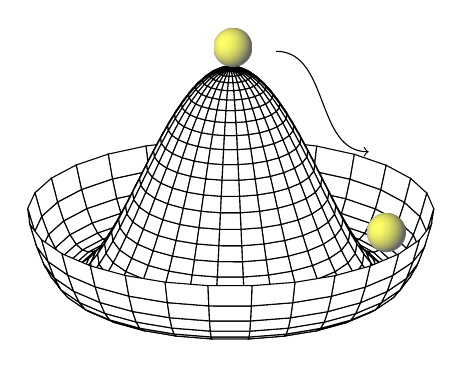
\begin{tikzpicture}
  \begin{axis}[
    hide axis,
    samples=30,
    domain=0:360,
    y domain=0:1.25
    ]
    \addplot3 [surf, shader=flat, draw=black, fill=white, z buffer=sort] ({sin(x)*y}, {cos(x)*y}, {(y^2-1)^2});
  \end{axis}
  \shade[shading=sphere] (3.45, 4.45) circle [radius=0.25cm];
  \shade[shading=sphere] (5.4, 2.1) circle [radius=0.25cm];
  \node[anchor=east] at (4.0, 4.4) (text) {};
  \node[anchor=south] at (5.3, 3.0) (description) {};
  \draw (description) edge[out=180, in=0,<-] (text);
\end{tikzpicture}
